\chapter{Time Delay Compensation and Predictive Display}
\label{ch_7:PDsply}
In the last chapter it was shown using simulation results that time delay between the remote and local station leads the system towards instability. In this chapter we first present predictive model controller for time delayed teleoperation. We then highlight the issues of time delay on human performance. We then present our  RGB-Depth sensor based  predictive display implemented in our system  to alleviate the problem of time delay in visual feedback.

\section {Model Based Time Delay Compensation}
As shown in the last chapter, simulation of time delays system with pure pursuit model for human controller in stability starts with as the delay in feedback i.e input delay to the human model increase. In paper by Ollero \cite{ollero1995stability} stability of pure pursuit with input delay was presented. The details of which is presented in Appendix \ref{appendix_b}.   In view of the above theoretical analysis and the simulation results presented in the last chapter its required to design  a stabilizing controller to take care of large delays i.e 0.8 sec. One such design based on model based predictive control is presented next.

 \begin{figure}
 	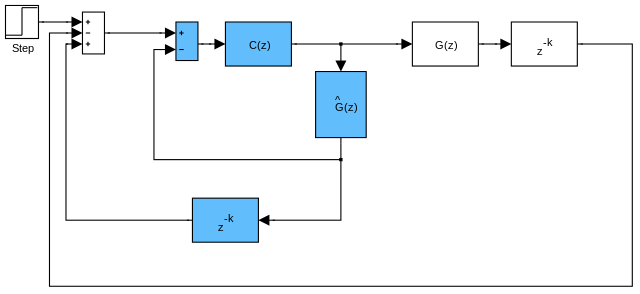
\includegraphics[width=\linewidth]{Chapter7/fig/Smith_predictor}
 	\caption{Smith Predictor}
 	\label{fig:Smith}
 \end{figure}
 
 One of the earliest predictor based controller for Linear system with time delay  was proposed by Smith \cite{smith1959controller} called the Smith Predictor or Smith Controller. The schematic of the smith controller is shown in figure \ref{fig:Smith}. There are two loops the inner and the outer loop. Where $G(z)$ is the plant, $C(z)$ is the stabilizing controller  for plant with out delay, $\hat{G}(z)$ is the model of the plant.  As can be seen from the figure \ref{fig:Smith} that during the period (k time unit ) when the feedback (output) is not available the model of the plant is used to predict the actual plant behaviour and generate the control signal accordingly. 
 
 In our case the plant is a mobile robot. The block digram shown in Figure \ref{fig:blockdigTimeDelay} depicts the architecture of the time delay system applicable to the current system. The teleoperation  over wireless network for our system   resulted in a delay of $T_1= 500~ms$, or update frequency of 2Hz,  for the video feedback from robot camera. This is due to the large amount of data being transmitted. The Figure \ref{fig:delayphoto} shows the measured delay in video link. The frequency of odometric and control  data exchange between the two stations was at the rate of 20Hz, ie a delay $T_2=50ms$. This  loop runs was independent of the video feedback link.  It may be noted that $T_2<<T_1$ for this system.
 \begin{figure}[ht]
 	\centering
 	\begin{minipage}{0.45\textwidth}
 		\centering
 		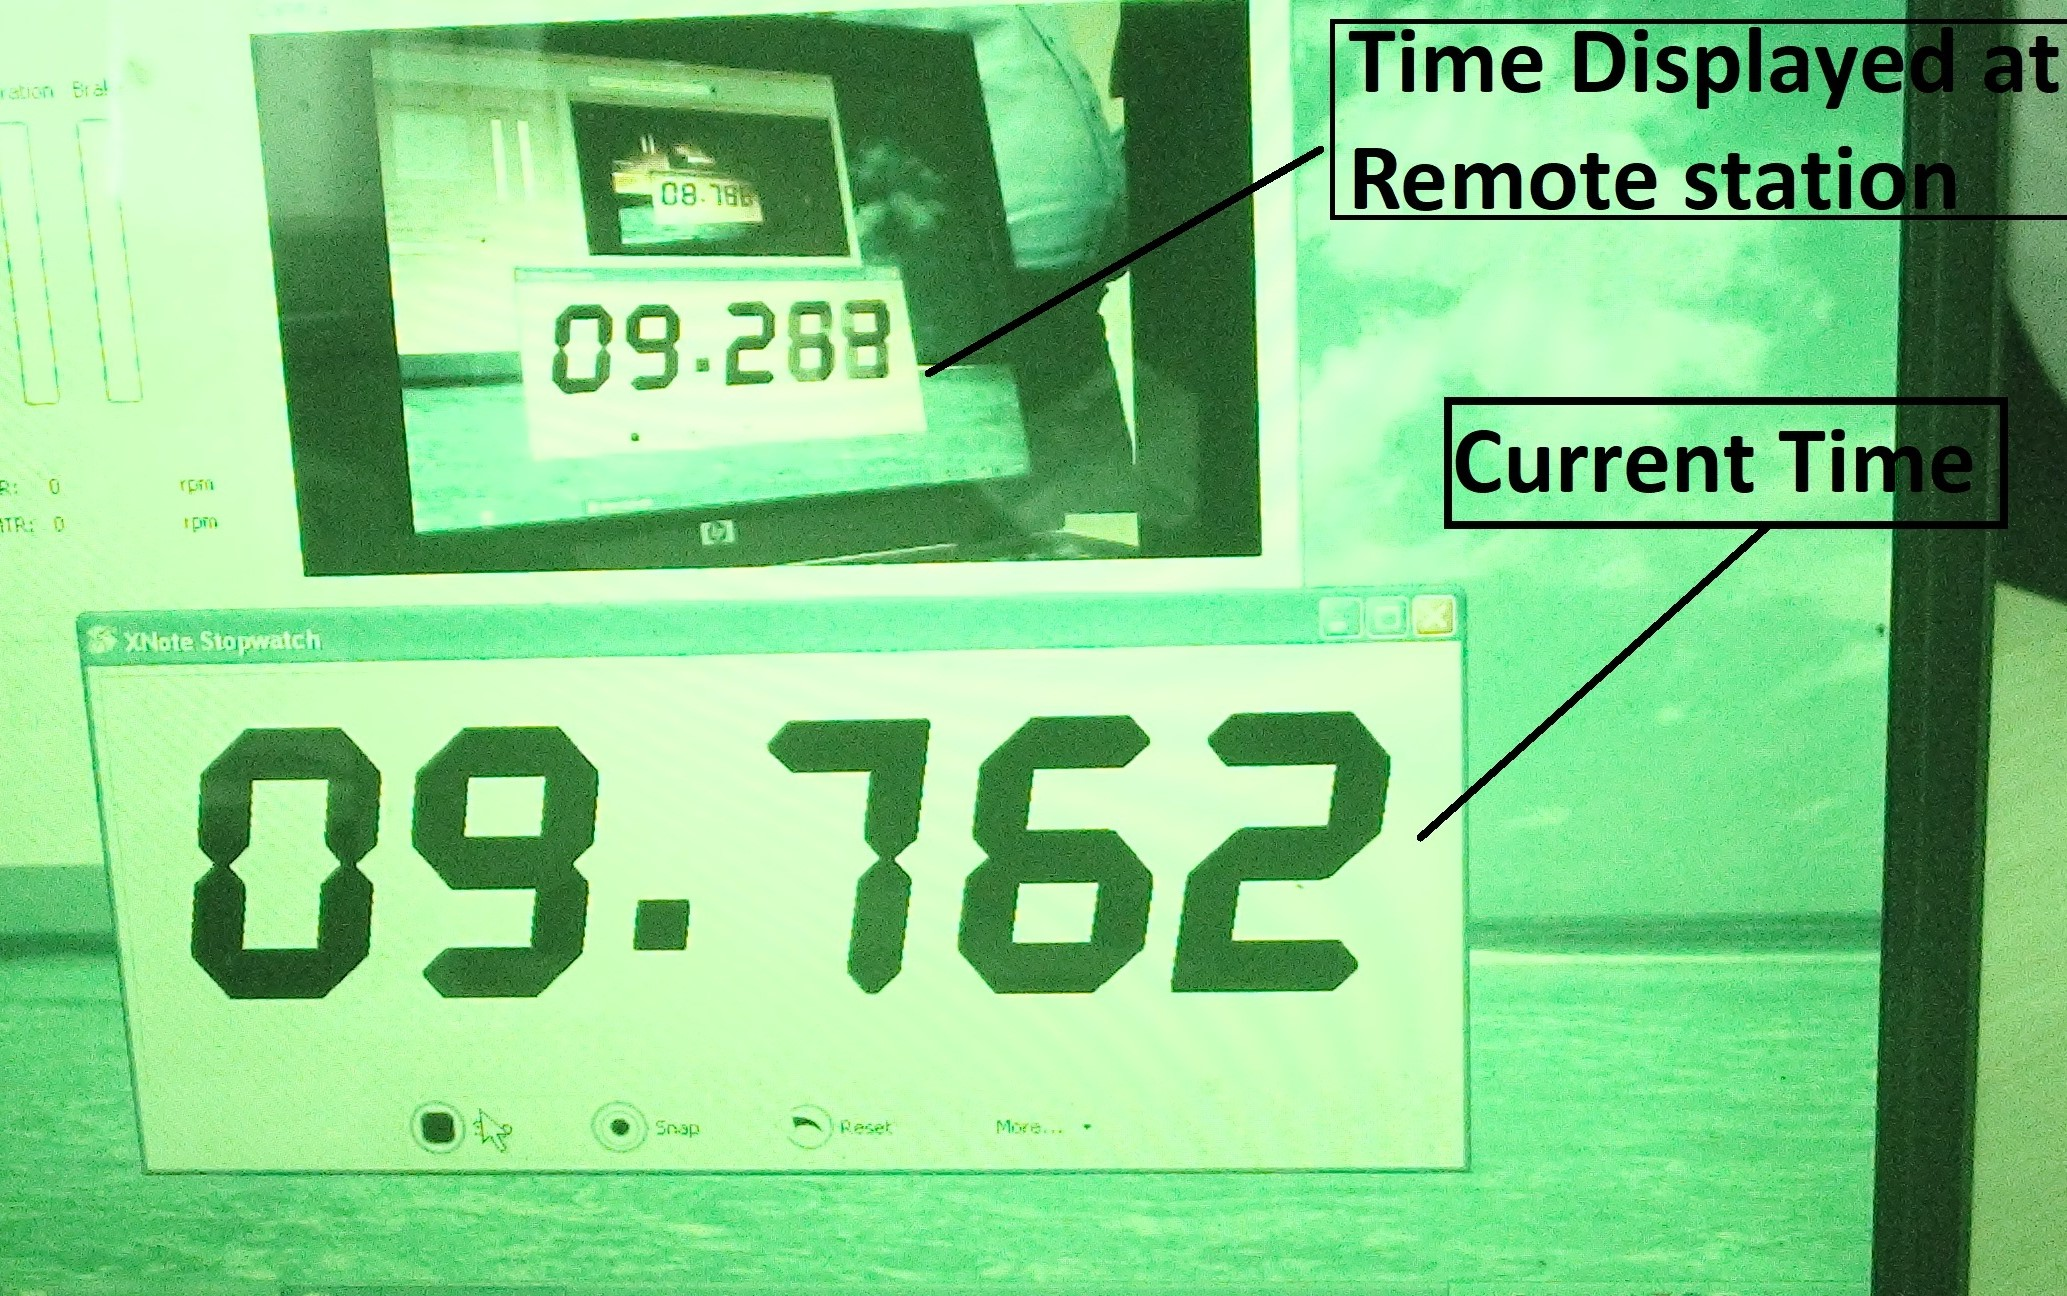
\includegraphics[width=\linewidth,keepaspectratio]{Chapter7/fig/delayMeasureNew}
 		\captionof{figure}{Delay measurment}
 		\label{fig:delayphoto}
 	\end{minipage}%
 	\begin{minipage}{0.55\textwidth}
 		\centering
 		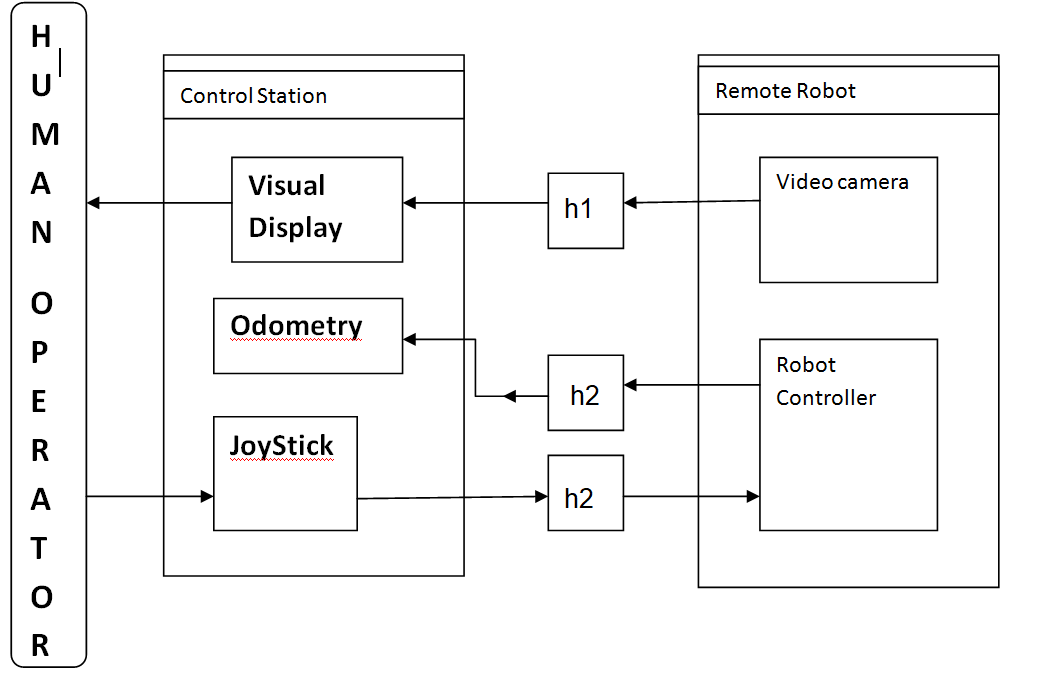
\includegraphics[width=.9\linewidth,keepaspectratio]{Chapter7/fig/BlockTimeDelay}
 		\captionof{figure}{Block digram of \\time delay system}
 		\label{fig:blockdigTimeDelay}
 	\end{minipage}
 \end{figure} 

%This was possible because  A new pose was predicted based on the odometric data and fed to the "human operator model" for the intermediate control action.
\subsection{Proposed Controller}
The proposed control strategy to mitigate the effect of time delay is to predict the current position based on the dynamic model of the mobile robot from the last known position from the delayed video image.  As shown in Figure \ref{fig:SmithRobot} let us assume that we are at time $t+\delta$, but the latest pose  data of the robot available is that of at time $t$. We predict the present pose i.e at time $t+\delta$ based on the dynamic model  of the robot derived in Chapter \ref{c4_Dynamics}, Equation \ref{CE}, and presented here again for convenience. 
\begin{equation}
\label{CE2}
\quad I(\theta)\ddot{\theta}=C(\theta,\dot{\theta})\dot{\theta}+\tau
\end{equation}
It may be noted that the dynamic model uses torque $\tau$ as it input. Where as the local station which uses, pure pursuit for sumulation of  human action,   generates Linear  $v$ and Angular $\dot\theta$  velocities of the robot as shown in Figure \ref{fig:SimBlock}. This is taken care by first converting $V \equiv\dot o_3$ and $\dot\theta\equiv\omega_3$ to rear wheel velocities using Equations \ref{omegaPlat} and \ref{velPlat}. The rear wheel velocities  are then used in PI controller given Chapter \ref{c5_Control} of the rear wheel motors to generate the $\tau$ for Equation \ref{CE2}.

This predicted position is given to the pure pursuit algorithm to generate required control outputs for the remote robot. In the simulation it is assumed that this control inputs reaches the remote robot instantaneously, as $T_1>> T_2$. As discuss in the Chapter \ref{c6_simulation}   Kinematic model given by Equation \ref{eqn:KinematicModelOfRobot} is used to simulate remote robot.
 \begin{figure}
	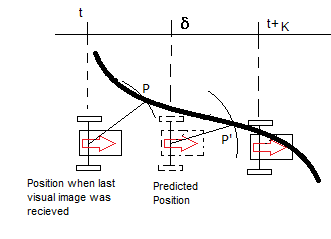
\includegraphics{Chapter7/fig/robotPredictPos}
	\caption{Smith predictor applied to mobile robot}
	\label{fig:SmithRobot}
\end{figure}

\subsection{Simulation algorithm and  results} 
The algorithm used in the simulation is given below.
The algorithm for simulation is explained in the following steps.
\begin{enumerate}
	\item Convert the path from global coordinate system (CS) to Robots Local Coordinate System
	\item With a given look ahead distance (l) search for a goal point on the path.
	\item Determine the turning radius (r) using Equation 6.5
	\item \label{command} Calculate the command to the robot based on Equation 6.6.
	\item Calculate the predicted pose of the robot  based on commanded given in Step \ref{command} and dynamic model of robot given in Equation \ref{CE2}.
	\item update robot pose $(x,y,\theta)$
	\item goto Step 1 
\end{enumerate} 

 Simulation was carried using Matlab. Differential equation solver \textit{"de24"} was used to solve equation \ref{eqn:KinematicModelOfRobot} and \ref{CE2}.  The desired path  was a circle of radius 5m centred at origin of the global coordinate system. The human action was modelled with look ahead distance $l$, of 0.5m and linear velocity $V$, of 0.5m/s. The initial position of the robot was (4.5,0.0).
 
 The  performance of the system with zero delay, i.e. $T_1=T_2=0$ is shown in Figure \ref{fig:nodelayplot}. Figures \ref{fig:PreDelay500plot} and \ref{fig:PreDelay800plot} show the   robot's motion under delay of 0.5 and 0.8 sec.  It is seen that oscillation are no more visible at 0.5sec delay and with the delay of  0.8 sec. The system shows no instability. 
 \begin{figure}[h]
 	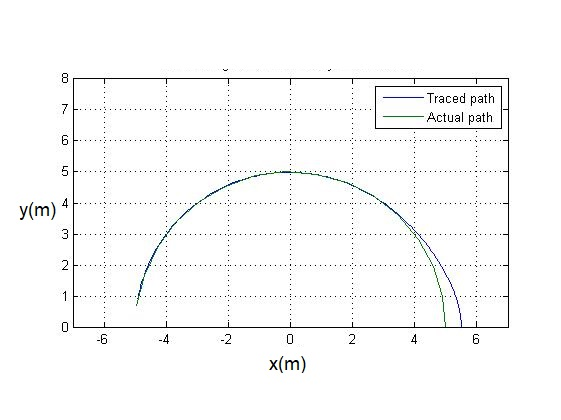
\includegraphics[width=\linewidth,keepaspectratio]{Chapter7/fig/withPrediction05dely}
 	\captionof{figure}{Simulation with  time delay $T_1=.5sec$ and $T_2=0$ }
 	\label{fig:PreDelay500plot} 
 \end{figure} 
 \begin{figure}[h]
 	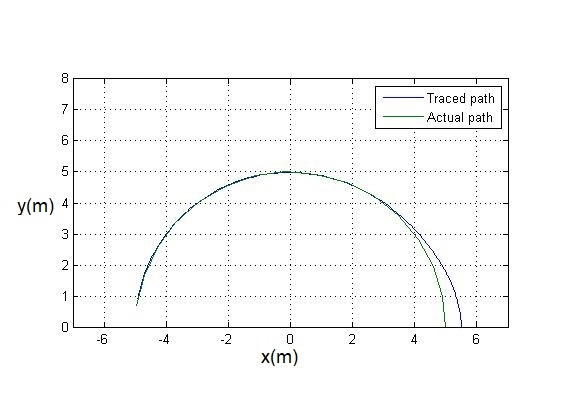
\includegraphics[width=\linewidth,keepaspectratio]{Chapter7/fig/withPrediction08delay}
 	\captionof{figure}{Simulation with  time delay $T_1=.8sec$ and $T_2=0$ }
 	\label{fig:PreDelay800plot} 
 \end{figure}
  
\section{Predictive Display}
Predictive display has been defined as using the computer for extrapolating the display forward in time \cite{sheridan}. In this a local model of the remote scene is used to predict and render the remote scene in response to operator command. It replaces the delayed video feedback with extrapolated synthesised  image of the remote environment and local enables the operator to perform the task normally. 

\section{Remote Scene Extrapolation} 
The visual data present in the current frame is the view that the robot has seen $h_1$ second earlier. In order to predict the current scene that the robot might be seeing we need to estimate the current position of the robot. Once the current position of the robot is known we re-construct a view form the old scene by moving the view point to the current position of the robot. To explain this further and to use it in the teleoperation simulation model discussed in chapter 6
\subsection{here}

